\subsection{Broadcast}

\begin{figure}[htb!]
  \centering
    \subfloat[]{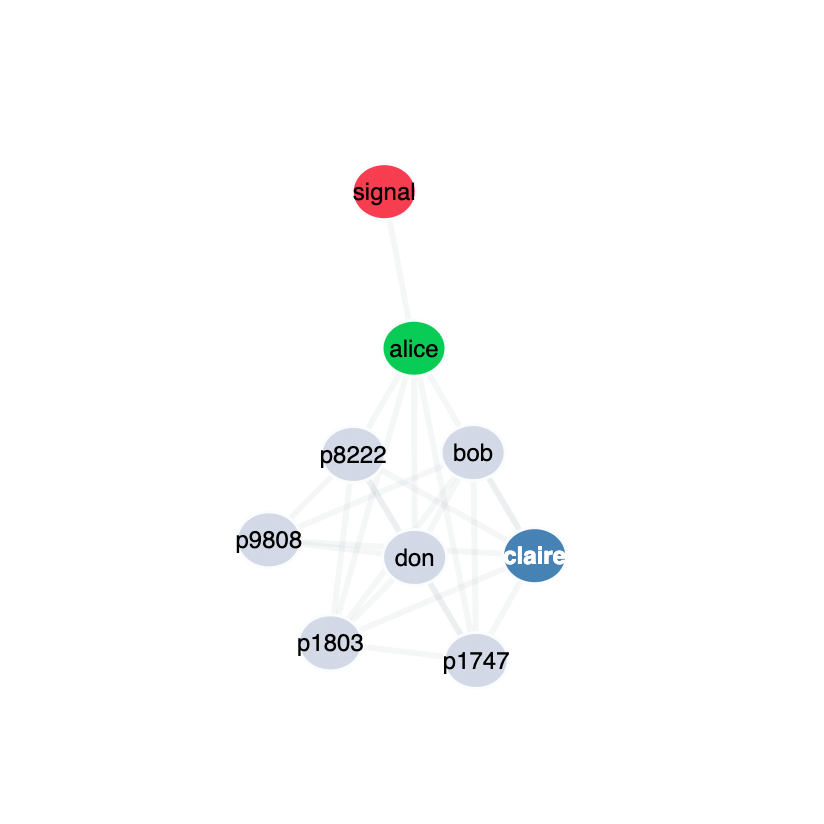
\includegraphics[width=0.25\textwidth]{graphics/analysis/mini-scenarios/stream/1.png} \label{fig:filmstrips-broadcast-a}}
    \subfloat[]{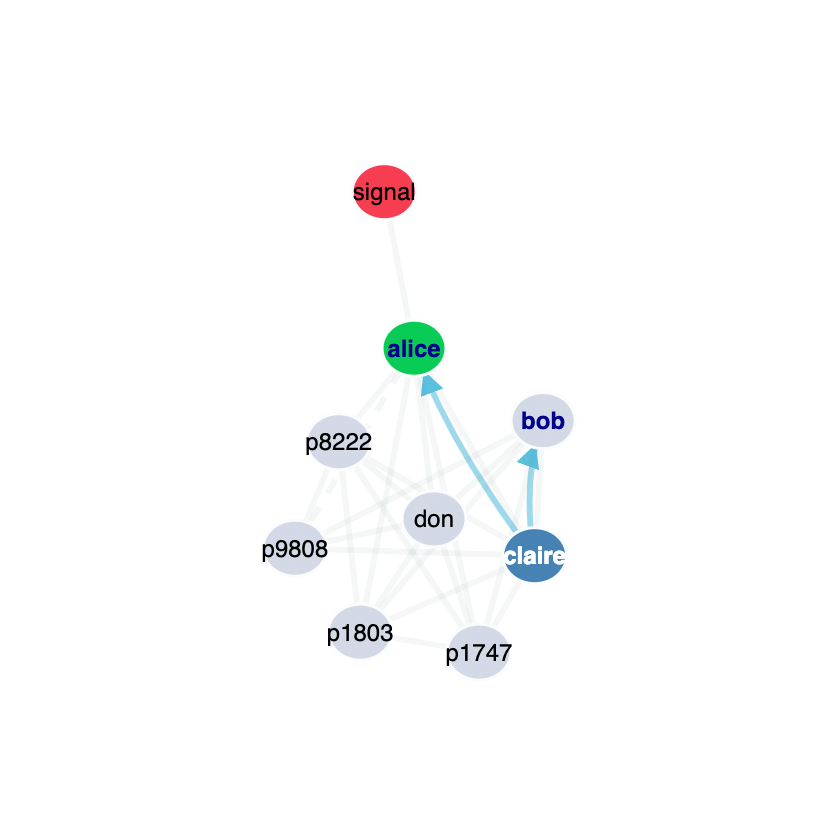
\includegraphics[width=0.25\textwidth]{graphics/analysis/mini-scenarios/stream/2.png} \label{fig:filmstrips-broadcast-b}}
	\subfloat[]{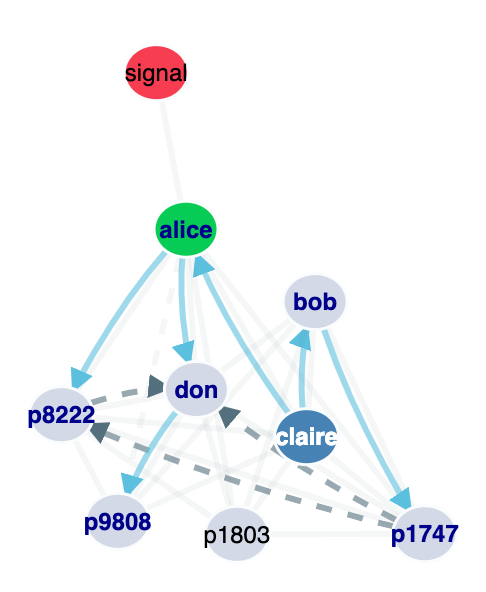
\includegraphics[width=0.25\textwidth]{graphics/analysis/mini-scenarios/stream/3.png} \label{fig:filmstrips-broadcast-c}}
	\subfloat[]{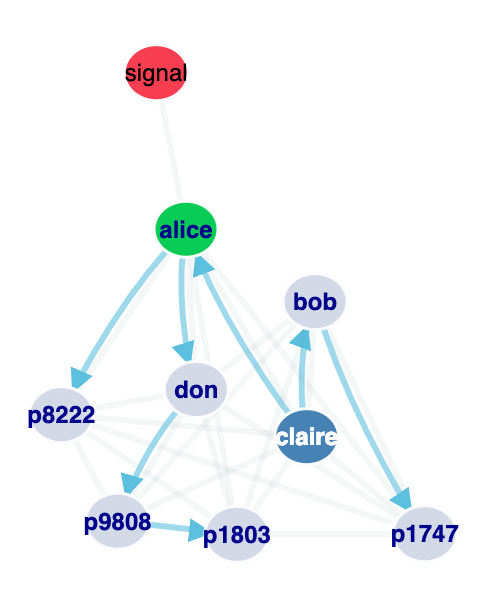
\includegraphics[width=0.25\textwidth]{graphics/analysis/mini-scenarios/stream/4.png} \label{fig:filmstrips-broadcast-d}}
	\caption{Broadcasting tree creation}
\label{fig:filmstrips-broadcast}
\end{figure}

This scenario shows how the video broadcast is propagated through the network. \claire is the peer who is starting a broadcast (\vref{fig:filmstrips-broadcast-a}). 
She is selecting her two best neighbours and starts the connection negotiation process to open a WebRTC Stream connection. 

By using the WebRTC Data connection and the Ping/Pong-messages she has measured that \alice and \bob are her best neighbours. They both accept the offer and reply with an answer. \claire establishes the connection and start sending them the video stream (\vref{fig:filmstrips-broadcast-b}).

In the meantime \alice and \bob are selecting their best neighbours to open a WebRTC Stream connection to rebroadcast the video stream from \claire. The process repeats until it has reached all peers. However, each peer accepts only one incoming WebRTC Stream connection and is only opening two outgoing.
In \vref{fig:filmstrips-broadcast-c} \don receives a broadcast offer from multiple peers. As he has already an incoming stream connection from \alice he is rejecting all offers.

Peers that have been left behind during the selection process receive \textit{Stream-Announcements} from their neighbours with the information how many free connections they have. \textit{p1803} has not be selected in the first phase but he receives a Stream-Announcement from his neighbours \claire, \don, \textit{p9808} and \textit{p1747}. \claire has no available connection thus it can only select \don, \textit{p9808} and \textit{p1747}. He sends all of them a WebRTC Stream connection request. \textit{p9808} replies with an offer first, thus \textit{p1803} opens a connection to this peer.
